\section{Reševanje enačb}
\label{pogl:enacbe}

% in kubične enačbe (operacija O7!), za bolj zahtevne pa bosta zanimivi podpoglavji o reševanju enačb 4.\ in 5.\ stopnje.
% Alhazijev al kej je že uni problem!!!

% - kubične enačbe
%     - z Belochinim kvadratom
%     - Lillova metoda (z Belochinim prepogibom)
%     - Alperinova rešitev (gl. Hull 2020)
% - enačbe 4. stopnje (TEŽJE) --> Alhazen's problem (gl.\ članek od Vavšetiča in tudi~\cite[str.\ 137--139]{geometricconstructions})
% - enačbe 5. stopnje (TEŽJE)

Zapustimo deloma področje geometrije in si poglejmo, kako lahko s prepogibanjem papirja rešujemo enačbe.

Linearne enačbe z racionalnimi koeficienti ni težko rešiti. Enačba $ax + b = 0$ ima rešitev $x = -b/a$. To je racionalno število, ki je po izreku~\ref{izr:origami_konstruktibilnost} origami-konstruktibilno.

Iz podpoglavja~\ref{podpogl:evkl_konstruktibilnost} vemo, da lahko z neoznačenim ravnilom in šestilom konstruiramo natanko števila oblike $a + b\sqrt{r}$, kjer so $a, b, r \in \Q$. Take oblike je tudi splošna rešitev kvadratne enačbe z racionalnimi koeficienti in ker lahko ta števila konstruiramo tudi z origamijem, lahko preko kvadratne formule najprej izračunamo realni rešitvi in ju nato s prepogibanjem papirja preko operacij seštevanja, odštevanja, množenja, deljenja in korenjenja konstruiramo (izrek~\ref{izr:origami_konstruktibilnost}). Zanima pa nas, ali jih je mogoče konstruirati tudi brez predhodnega računanja.

V tem poglavju si bomo pogledali, kako z origamijem na prefinjen način -- brez konstrukcije preko zgornjih petih operacij -- rešujemo enačbe druge, tretje, četrte in pete stopnje. Vedno bo veljalo, da imamo za $n$-to stopnjo, kjer je $n \in \{2, 3, 4, 5\}$ dano enačbo
$$ a_n x^n + a_{n-1} x^{n-1} + \ldots + a_2 x^2 + a_1 x + a_0 = 0, $$
kjer so $a_i \in \Q$ za vsak $i \in \{1, 2, \ldots, n\}$ in $a_n \ne 0$. Da se znebimo enega koeficienta, lahko enačbo brez škode za splošnost delimo z vodilnim koeficientom $a_n$, saj s tem koeficienti ostanejo racionalni. Zato od zdaj naprej predpostavimo $a_n = 1$.

Spomnimo se še, da smo origami-konstruktibilna števila definirali kot vsa števila, ki jih lahko s prepogibanjem konstruiramo preko na začetku dane abscine osi, izhodišča $(0,0)$ in točke $(1,0)$ in da lahko kar predpostavimo, da imamo dan celoten koordinatni sistem z abscisno in ordinatno osjo, izhodiščem ter enoto $1$ na obeh oseh (definicija~\ref{def:origami_konstruktibilnost}). 

\subsection{Kvadratna enačba}

Uporabimo kar standardne oznake za koeficiente kvadratne enačbe, torej rešujemo enačbo oblike
\begin{equation}
    \label{eq:spl_kv_en}
    x^2 + bx + c = 0
\end{equation}
Predpostavimo, da ima enačba dve različni realni rešitvi oz.\ da je diskriminanta enačbe pozitivna, t.\ j.\ $D = b^2 - 4c > 0$. Če realnih ničel ni, o origami konstrukciji rešitev namreč nima smisla razpravljati. Če je rešitev ena, je podana kot $x = -b/2$, kar je origami-konstruktibilno število in se ga takoj konstruira.

Enačba~\ref{eq:spl_kv_en} nam poda pokončno parabolo $y = x^2 + bx + c$ z vodoravno premico vodnico in dvema ničlama, ki sta rešitvi naše enačbe. Iščemo absciso presečišča parabole z abscisno osjo.

Zopet se bomo poslužili dosedanjega znanja o operaciji~\ref{op:O6}. Ta nam s pregibom skozi dano točko $B$, ki točko $A$ položi na premico $a$, konstruira tangento na parabolo z goriščem v točki $A$ in premico vodnico $a$.

Naša parabola je z enačbo seveda natančno določena. Ideja iskane konstrukcije rešitev enačbe je določiti tako točko $B$ (najlažje kar na osi parabole), da bi nam izvedba operacije~\ref{op:O6} podala tangento na parabolo ravno v njeni ničli. Želeni pregib mora potekati skozi točko $B$ in gorišče $A$ položiti na tisto točko $A'$ na premici vodnici $a$, ki ima enako absciso kot ničla parabole. (gl.\ sliko~\ref{fig:tockaB_in_O6}). Taka točka $B$ je z osjo parabole in katerokoli izmed ničlama (zaradi simetrije) natanko določena.

\begin{figure}[h]
    \centering
    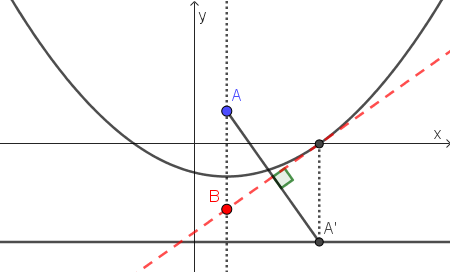
\includegraphics[width=0.5\textwidth]{images/kvadratna_enacba/tockaB_in_O6.png}
    \caption[Iskanje točke $B$]{Operacijo~\ref{op:O6} skozi iskano točko $B$ poda rešitev kvadratne enačbe.}
    \label{fig:tockaB_in_O6}
\end{figure}

Edina nevarnost, da ta konstrukcija ne bo delovala, je možnost, da točka $B$ kdaj ne bo origami-konstruktibilna točka. Zato sedaj izračunajmo njene koordinate in se prepričajmo, da se to nikoli ne bo zgodilo.

Najprej iz dane enačbe parabole določimo njeno gorišče $A$ in premico vodnico $a$. Spomnimo se, da iz enačbe parabole oblike
$$ (x - x_0)^2 = 2p(y - y_0) $$
takoj razberemo koordinati gorišča $(x_0, y_0)$ in enačbo premice vodnice $y = y_0 - p$. V našem primeru enačbo $y = x^2 + bx + c$ preoblikujemo v
$$ \left(x-\left(-\frac{b}{2}\right)\right)^2 = 2 \cdot \frac{1}{2} \left(y - \left(c - \frac{b^2}{4}\right)\right). $$
S tem sta gorišče $A$ in premica vodnica $a$ določena:
$$ A\left(-\frac{b}{2}, c - \frac{b^2 - 1}{4}\right) \text{ in } a: y = c - \frac{b^2 + 1}{4}. $$

Naj bo $t$ ena izmed rešitev enačbe~\ref{eq:spl_kv_en}. Na premici $a$ z $A'$ označimo točko z absciso $t$. Poiščimo enačbo pregiba, ki gorišče $A$ položi v točko $A'$. Ta pregib bo tangenten na parabolo ravno v njeni ničli, njegovo presečišče z osjo parabole $ x = -b/2 $ pa nam bo določilo točko $B$.

Koeficient nosilke daljice $AA'$ je $ - 1/(2t + b)$, torej je koeficient pregiba $k = 2t + b$. Pregib je po konstrukciji tangenten na parabolo v ničli $(t, 0)$, torej je njegova enačba
$$ y = (2t + b)(x - t) = (2t + b)x - 2t^2 - bt = (2t + b)x - t^2 + c. $$
Pri tem smo upoštevali, da velja $t^2 + bt + c = 0$. Presečišče pregiba in osi parabole je tako točka $B$ z absciso $ x = -b/2 $ in ordinato
$$ y = (2t + b)\left(-\frac{b}{2}\right) - t^2 + c = - t^2 - tb + c - \frac{b^2}{2} = c + c - \frac{b^2}{2} = 2c - \frac{b^2}{2}.$$
Obe koordinati sta racionalni, torej je točka $B$ konstruktibilna točka. Ker leži na osi parabole, nam poda obe rešitvi enačbe -- pregiba sta si simetrična glede na os. Povzemimo sedaj postopek konstrukcije rešitve kvadratne enačbe~\ref{eq:spl_kv_en}:
\begin{enumerate}
    \item V koordinatnem sistemu konstruiramo gorišče $A\left(-\frac{b}{2}, c - \frac{b^2}{4} + \frac{1}{4}\right)$, premico vodnico $a: y = c - \frac{b^2}{4} - \frac{1}{4}$ in točko $B(-\frac{b}{2}, 2c - \frac{b^2}{2})$.
    \item Z operacijo~\ref{op:O6} naredimo pregib skozi točko $B$, ki točko $A$ položi na premico $a$ (če je diskriminanta enačbe pozitivna, sta možna pregiba dva).
    \item Skozi sliko točke $A$ naredimo vertikalen pregib in njegovo presečišče z abscisno osjo nam konstruira ničlo dane enačbe.
\end{enumerate}

\textbf{Primer:} Poiščimo rešitve enačbe $x^2 - x - 1 = 0$. Določimo obe točki in premico: $A(\frac{1}{2}, -1)$, $B(\frac{1}{2}, -\frac{5}{2})$ in $a: y = -\frac{3}{2}.$. Opravimo operacijo~\ref{op:O6} in označimo presečišče abscisne osi in pravokotnice nanjo skozi sliko točke $A$. Če smo bili pri pregibanju natančni, dobimo presečišči pri $x_{1,2} = \frac{1 \pm \sqrt{5}}{2}$ (gl.\ sliko v~\cite[str.\ 37]{hull2020}).

To še zdaleč ni edini postopek za reševanje kvadratne enačbe. Kot še en lep primer Hull v\~cite[str.\ 38]{hull2020} navaja Lillovo metodo, dokaz pa prepušča bralcu. Ta metoda je tudi zgled, kako lahko najprej najdemo evklidsko konstrukcijo rešitev kvadratne enačbe in jo nato preobrazimo v origami konstrukcijo -- saj že vemo, da lahko s prepogibanjem papirja konstruiramo vse in še več, kar se da z evklidskim orodjem.

\subsection{Kubična enačba}

% operacija O7??
% z Belochinim kvadratom
%     - Lillova metoda (z Belochinim prepogibom)
%     - Alperinova rešitev (gl. Hull 2020)

Za kubične enačbe iz parabol (kar sledi iz operacije~\ref{op:O7}) lahko gledaš~\cite[str.\ 150]{geometricconstructions}.

\subsection{Kvartična enačba}

\subsection{Kvintična enačba}